%!TEX root = ../template.tex

\chapter{Approach to Elaboration Phase}
\label{cha:approach_to_elaboration_phase}

This chapter presents an overview of the planned elaboration phase. 
In section \ref{sec:refinement_of_objectives_and_contributions} the objectives and contributions are more refined and matched against the related work discussed in chapter \ref{cha:related_work}, also discussing the scenario and environment where the system should fall.
Section \ref{sec:system_model_approach} presents a reference of the system model and blueprint architecture of the targeted solution. The architecture and implementation guidelines of the solution are approached in section \ref{sec:planned_architecture_and_implementation}.

After exposing the planned implementation and architecture, section \ref{sec:planned_testbench_environments} explains how and where it is planned to test the system, whereas section \ref{sec:relevant_evaluation_criteria} will complement it with what metrics will be gathered and how they will be compared with each other.

\section{Refinement of Objectives and Contributions} % (fold)
\label{sec:refinement_of_objectives_and_contributions}

The goal of this dissertation as explained on chapter \ref{cha:introduction}, is the design, development and validation with experimental evaluation of a secure in-memory storage (based on a "key-value" model), supported by a hardware-enabled trust computing base.

Regarding the security assumptions, the solution will provide: (i) hardware-isolated in-memory processing engine, designed as a hardware-isolated container (docker) facility, enclaved within the Intel-SGX protection guarantees; (ii) hardware-isolated communication endpoints for client access, providing TLS tunnelling with strong TLS 1.3 endpoint encryption parameterisations and support for mutual client/server authentication, and (iii) privacy-enhanced operations to be directly processed on encrypted data sets in memory. The former facility is particularly interesting to combine the possibility to manage protected memory for small data sets and also searchable encrypted data sets that are far larger than the protected memory limits imposed by the SGX memory mapping facility. Furthermore, the solution will target main data structures commonly use fine-grained data items that can include pointers, complex composite types and keys, which do not match well with the coarse-grained paging of the SGX memory extension technique.

In the next subsections we will align the implementation ideas starting by refining the circumvention of limitations in SGX and the threat model assumptions to address our solution.

\subsection{\gls{SGX} Limitations Refinement}
\label{ssec:sgx_limitations_refinement}

Section \ref{ssec:circumvention_of_sgx_limitations} describes in detail the limitations of \gls{SGX}. In our approach we will intend to design a solution that can be leveraged from conventional reference KVS technology, giving the possibility to manage small datasets but also larger datasets (directly mapped in non-protected memory). To circumvent the problem our solution must combine the possibility to use the internal capabilities native to SGX with the possibility of supporting operations managing datasets encrypted in memory, with such operations executed directly over encrypted data. This facility will be provided by the use of partial homomorphic encryption constructions, with data initially encrypted and submitted to the key-value-store solution with cryptographic keys only managed in the client side. Our solution will be designed in order to be possible the support for fine-grained key-value encryption, driven form the application requirements. Our target is the support of a variety of operations provided in a typical KVS API, taking REDIS as the reference solution and in order to support a considerable number of queries currently used by many REDIS-supported applications.

\subsection{Adversary Model}
\label{ssec:adversary_model}

As the baseline, our threat model will lie on the protection overview stated in SGX’s paper \cite{sgx:7}: \textit{SGX prevents all other software from accessing the code and data located inside an enclave including system software and access from other enclaves. Attempts to modify an enclave’s contents are detected and either prevented or execution is aborted}, which falls in the following adversary model:

\textbf{Isolation by trusted containerisation from malicious code}: The system performs and protects its data from an attacker capable of compromising the system through another application installed on the same system or malicious code existent or injected in the OS or OS hypervisor layers;

\textbf{Privacy protection against insider "Honest but Curious" System Administrators}: The system must be able to protect from an attacker with root access to the machine, with permissions to access and monitor memory-mapped data. This is relevant because we will target our solution as a candidate solution to protect data privacy in a cloud-based key value store solution as a service, preventing data-leakage vulnerabilities exploitable by insider incorrect users or system-administrators.

\textbf{Network Attacks:} All communication to and from the system (supporting client-service operations) should be secure, using proper strong cryptographic parameterisations for TLS 1.3, mutual authenticated handshakes and TLS endpoint executions isolated in SGX-enabled TLS tunnels in communication containers, avoiding attacks against the authentication of the service endpoints, as well as, attacks against the integrity and confidentiality of data flows supporting \gls{REST}/\gls{HTTPS} operations.

\textbf{File system and memory access attacks:} All sensitive data residing outside protected memory should be encrypted and operated in the encrypted form. An attacker can access the physical disks and hardware without the sensitive data being exposed.

\subsection{Other System Assumptions}
\label{ssec:other_system_assumptions}

With the above security baseline considered for the threat model assumptions, the solution must be  resilient to malicious privileged attacks and certain physical attacks. With a controlled and reduced hardware-shielded trust computing base, we want to design a solution that does not rely on the security of operating system managed by cloud providers. Furthermore, our solution must be also resilient to direct conventional physical attacks, such as cold boot attacks, which attempt to retain the DRAM data by freezing the memory chip or even bus probing to sense and to read exposed memory channel between the processor and memory chips. The only weaknesses not covered in our concerns with be the SGX  lack of protection for side-channel attacks.

The system planned has certain assumptions and aspects that are considered to be out of scope for this dissertation:

\begin{itemize}
	\item \textbf{Trusted Client} - The client side is assumed to be completely trusted and correct.
	\item \textbf{\gls{DoS} and \gls{DDoS}} attacks are out of scope.
	\item \textbf{Side Channel Attacks} - It is out of scope any side channel attacks or any related attack not present in \gls{SGX}'s threat model.
	\item \textbf{Physical and Hardware attacks} exploring the \gls{SGX} processing model and its isolation guarantees are out of scope, namely those presented above initially addressed in chapter \ref{cha:related_work}, section \ref{sec:trusted_computing _environments}.
\end{itemize}

\section{System Model Approach} % (fold)
\label{sec:system_model_approach}

The main goal of this project is modelled in figure \ref{fig:syste_model_detailed}. As shown, the model can be divided in three main components - the \textbf{client} which was already defined as trustable, the \textbf{communications} and the \textbf{backend service}. 

\begin{figure}[htbp]
  \centering{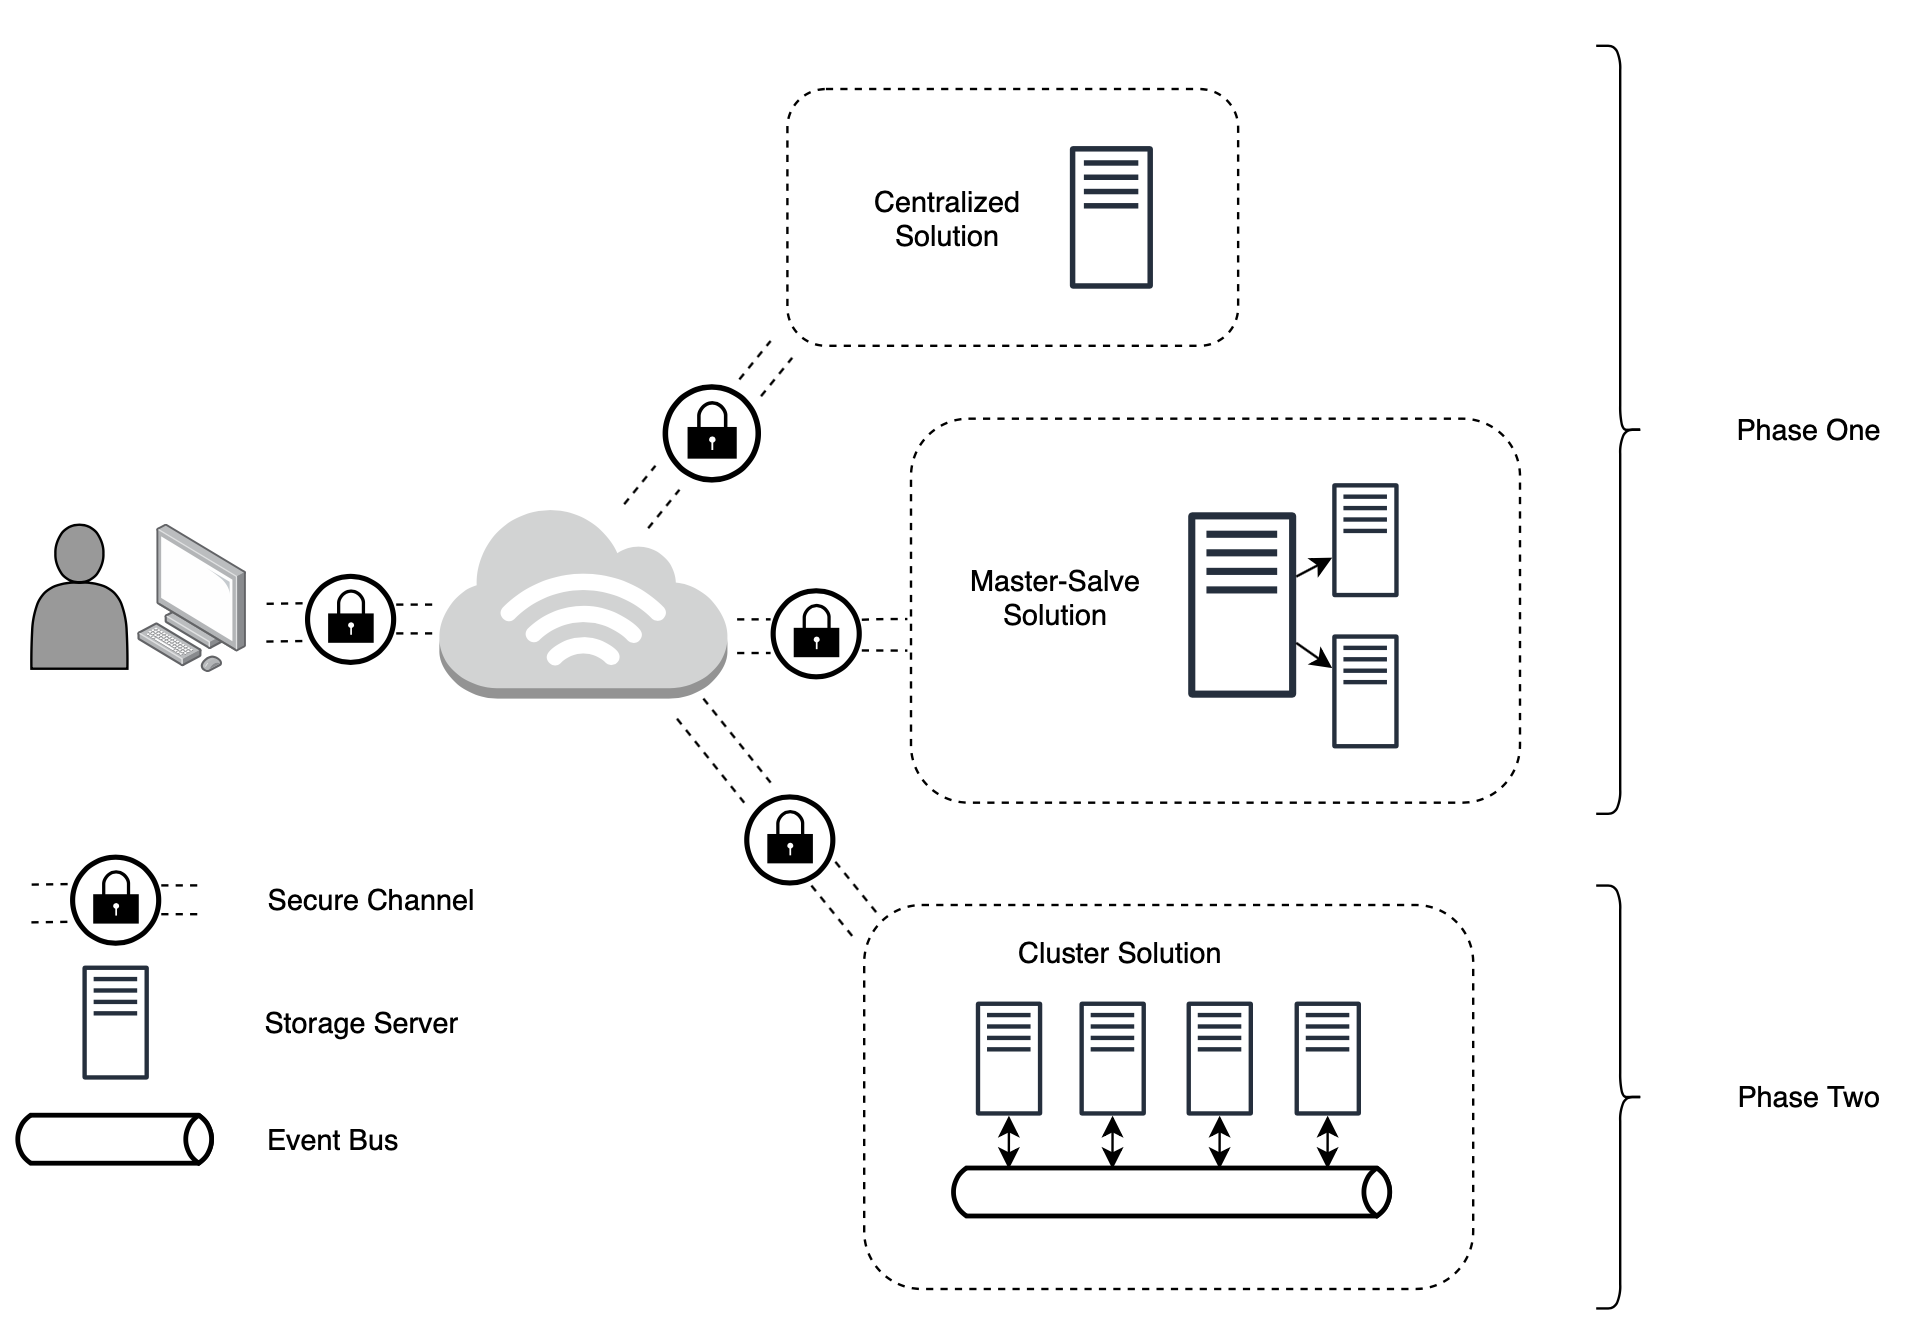
\includegraphics[width=0.9\linewidth]{SystemModelDetailed}}%
  \caption{System Model Details}
  \label{fig:syste_model_detailed}
\end{figure}

The system should comply with the adversary and threat model explained in section \ref{ssec:adversary_model}. The user should not be aware of implementation details and should have seamless interaction with the system despite the architecture and implementation provided by the backend, meaning that all solution should expose the same \gls{API} and support an interface as equal as possible to the unprotected version of the Key-Value Store. We must mention that the above system model will address the replication facilities as leveraged from the REDIS solution and trying to offer the same availability conditions as the original REDID cluster service. This availability provided by the replication of REDIS instances that can run as cloud service instances (that can be distributed among different cloud providers and geo-replicated datacenters) only offers consistency guarantees under a fail-stop model (not extended to byazntine-fault-tolerance or byzantine intrusion tolerance, that are conditions out of scope of our planned dissertation).

\section{Planned Architecture and Implementation} % (fold)
\label{sec:planned_architecture_and_implementation}

Cloud providers offer their services and applications in different stacks and computing infrastructures. They can be categorised in two main and most common: \gls{IaaS} (Infrastructure as a Service), and \gls{SaaS} (Software as a Service). These are terms to represent how much of the stack is available for user customisation and how much is managed by the provider. Figure \ref{fig:computing_stacks} shows the two stacks that where the shaded components represent the ones managed by the provider.

\begin{figure}[htbp]
  \centering
  \subcaptionbox{IaaS Stack\label{fig:iaas_stack}}%
    {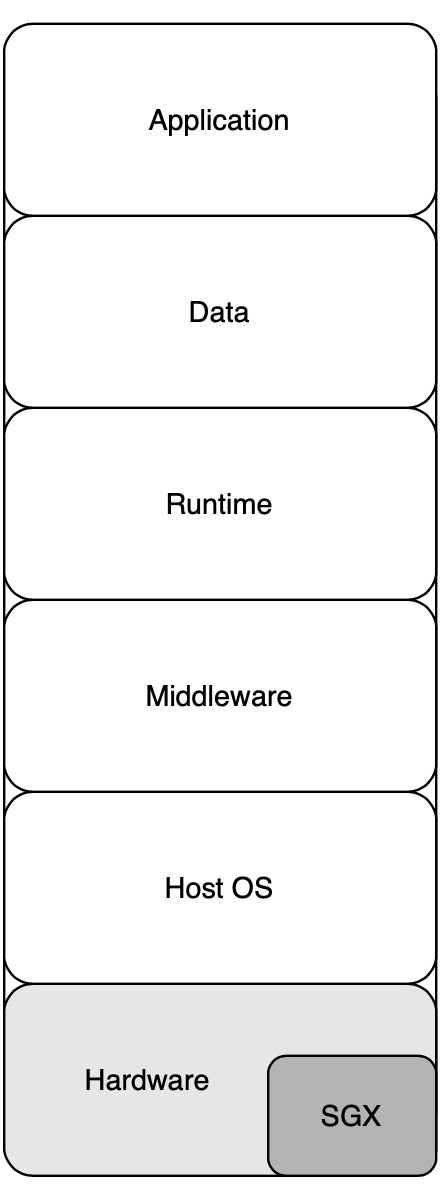
\includegraphics[width=0.2\linewidth]{IaaS_stack}}%
    \hspace{5em}
  \subcaptionbox{PaaS Stack\label{fig:saas_stack}}%
    {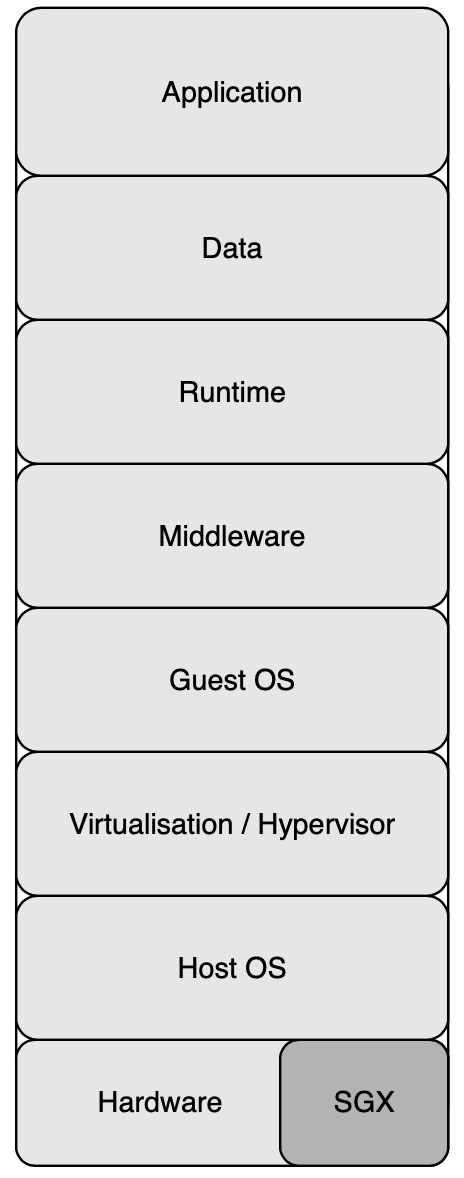
\includegraphics[width=0.2\linewidth]{SaaS_stack}}%
  \caption{Computing Stacks}
  \label{fig:computing_stacks}
\end{figure}

We will start development with a stack like figure \ref{fig:iaas_stack} as it is the simpler to customise and change to our needs especially for development. Everything besides the physical hardware can be customisable and it is managed by the user. In the end, we would like to expose the solution as a \gls{SaaS}, like figure \ref{fig:saas_stack} where it provides to the user a more abstracted environment, requiring less knowledge of computing bases and setups \cite{computing_stacks:1}.

As shown on figure \ref{fig:computing_stacks} and to achieve the objectives and goals of the project (\ref{sec:objectives_and_planned_contributions}), the hardware chosen was Intel's \gls{SGX} secure module. As explained in section \ref{ssec:intel_sgx}, this technology has the means and the ability to provide a truly isolated environment has required in this dissertation. The stack will be running a Linux Ubuntu Server \cite{ubuntu_server:1} operating system as the Host \gls{OS}, version 18.04 LTS. This version has compatibility with Intel's \gls{SGX} hardware, with the help of its \gls{SDK} and drivers \cite{sgx_sdk:1, sgx_drivers:1} and with some software needed in another layer of the stack.

Redis (v5.0.7 \cite{redis:1}) will be the key-value store application that will be worked on. This is the most used and most known \gls{KVS} technology, written in C language and will be deployed on the application component of the stack. To support large datasets, given \gls{SGX} limitations explained in section \ref{ssec:circumvention_of_sgx_limitations}, all data will be kept outside the enclave and will always be encrypted. The client can then decide to perform queries in encrypted form directly over the encrypted memory, sparing encryption and decryption cycles on the server. This will speed up the performance and will keep encryption keys away from the server in the cloud. Keys would be managed by the client which is considered trustable by the scope of this dissertation. Although this technique should help performance, it also means that system can lose some abilities and a set of operations. Fully homomorphic encryption is not feasible yet, so this solution will not be a full fledged solution. To this end, the solution will use the HomoLib, which is a JAVA Partial Homomorphic Cryptographic Library developed be the NOVA LINCS Research Center \cite{homolib:1}.

To help with \gls{SGX} integration a middleware software called Graphene \cite{graphene:1, graphene:2} will be used. This technology is a library \gls{OS} that \textit{"with \gls{SGX} support (...) can secure a critical application in a hardware-encrypted memory region. Graphene can protect applications from a malicious system stack with minimal porting effort"}. This library has already been tested with Linux Ubuntu Server 18.04 running as the \gls{OS}. 

Communications will be secure with the help of SGXStunnel \cite{sgxstunnel:1}, a prototype proxy to support TLS tunnelling with endpoints executed in a trusted execution environment provided by Intel SGX. \gls{SGX} termination means that at no time the data exchanged between the client and the server is exposed in clear text to any outsider because the packets are decrypted inside the secure module, which allows the network drivers, modules and physical cards to be removed from the \gls{TCB}.

Services and runtime environments will be coded using Java (Java SE 11 (LTS)) and the deployment of all softwares and services will be done with containers using docker technology \cite{docker:1}. Graphene already supplies integration with docker \cite{graphene_container:1}.

\section{Planned Testbench Environments} % (fold)
\label{sec:planned_testbench_environments}

The services will be deployed and tested in two different environments. The \textbf{development environment} translates to a local virtual machine that aims to simulate and be as close as possible to the production environment, but providing ease of development and rapid deployments. The \textbf{production environment} corresponds to a cloud provider that offers \gls{SGX} dedicated hardware, like OVHcloud \cite{ovhcloud:1}. The machines used should have the following specs:

\lstset{numbers=none, caption=Machine Specifications, label=lst:machine_specs}
\begin{lstlisting}
Dedicated Server Node
Processor: Intel 2x Xeon Silver 4214 - 24c/48t - 22.GHZ/3.2Ghz
Memory: 192 GB
Hard Drive: NVMe, SATA available
Public Network: Beginning at 1 Gbps
Private Network: Beginning at 2 Gbps
CloudLinux (Ubuntu 18.4 LTS Server 64 bits)
\end{lstlisting}

The tests will pe performed by a combination of the built-in Redis-Client benchmark tests \cite{redis_benchmark_cli:1} and to eliminate any bias claims, an external tester like the Yahoo! Cloud Serving Benchmark \cite{yahoo_benchmark:1}.

\section{Relevant Evaluation Criteria} % (fold)
\label{sec:relevant_evaluation_criteria}

The testers and benchmark clients will evaluate metrics that can be compared with a non secure solution. On the network layer, latency and throughput (as operations per seconds (ops/s)) and on the server side we will monitor the resources of the machines, like memory consumption, CPU load and also power consumption during the performance tests. Resource monitoring metrics should be gathered by the built in Linux tools like \textit{htop}, \textit{lsof} or \textit{vmstat}, and/or docker built-in tools like \textit{docker stats}.